% !TeX program = xelatex
% Сборка (рекомендуется, кириллица из коробки): xelatex article.tex
% Альтернатива: pdflatex --- нужен полный TeX Live с babel-russian и lh/cm-super (T2A).
\documentclass[a4paper,12pt]{article}

\usepackage{fontspec}
\usepackage{polyglossia}
\setdefaultlanguage{russian}
\setotherlanguage{english}

\usepackage{amsmath}
\usepackage{array,booktabs,etoolbox,geometry,graphicx,microtype,indentfirst,textcomp}
\usepackage{tikz}
\usetikzlibrary{arrows.meta,positioning}
\geometry{hmargin=2.5cm,vmargin=2cm}
% Системный шрифт с кириллицей (на macOS обычно есть Arial / Times New Roman).
\setmainfont{Arial}
\setmonofont{Arial}[Scale=0.92]

\setlength{\parindent}{1.25cm}
\sloppy

\title{Процедурная мета-рефлексия для генеративных языковых моделей}
% Аффилиация = место учёбы / работы (организация, город, страна).
\author{%
  Муляр Александр Евгеньевич --- студент 2-го курса, факультет <<ИИКС>>, Национальный исследовательский ядерный университет <<МИФИ>>, Россия, г.~Москва; \texttt{sshmulyar@gmail.com}\\[0.45em]
  \textit{Соавтор:} Душкин Роман Викторович --- старший преподаватель кафедры №~22, Национальный исследовательский ядерный университет <<МИФИ>>, Россия, г.~Москва
}
\date{}

% В стандартном article \maketitle вставляет \newpage до и внутри \@maketitle — из-за этого
% появляется пустая страница перед титулом; блок автора выносится из center во flushright с minipage для переносов и выравнивания по правому краю.
\makeatletter
\patchcmd{\@maketitle}{%
  \newpage
  \null}{%
  \null}{}{}%
\patchcmd{\maketitle}{%
      \if@twocolumn
        \ifnum \col@number=\@ne
          \@maketitle
        \else
          \twocolumn[\@maketitle]%
        \fi
      \else
      \newpage
        \global\@topnum\z@   % Prevents figures from going at top of page.
        \@maketitle
      \fi}{%
      \if@twocolumn
        \ifnum \col@number=\@ne
          \@maketitle
        \else
          \twocolumn[\@maketitle]%
        \fi
      \else
        \global\@topnum\z@   % Prevents figures from going at top of page.
        \@maketitle
      \fi}{}{}%
\patchcmd{\@maketitle}{%
    \vskip 1.5em%
    {\large
      \lineskip .5em%
      \begin{tabular}[t]{c}%
        \@author
      \end{tabular}\par}%
    \vskip 1em%
}{%
    \vskip 1.5em%
\end{center}%
\begin{flushright}%
\begin{minipage}{0.92\linewidth}%
\raggedleft
{\large
\lineskip .5em
\@author\par}%
\end{minipage}%
\end{flushright}%
\begin{center}%
    \vskip 1em%
}{}{}%
\makeatother

\begin{document}
\maketitle
\thispagestyle{empty}

\section*{\textit{Аннотация}}
\textit{%
Генеративные языковые модели нередко выдают содержательный ответ при низкой прозрачности выбранной процедуры и условий её переноса на близкие постановки. Предлагается процедурная мета-рефлексия: до вычислений --- явная классификация задачи и обоснованный выбор процедуры с отвергнутыми альтернативами; в ходе решения --- процедурная аннотация шагов и маркировка точек адаптации; после ответа --- ретроспекция применимости и переносимости. На открытом стенде PMR-Bench из десяти прикладных задач в четырёх предметных доменах выполнено парное сравнение целевого промпта со структурированным базовым условием без мета-рефлексии на одних и тех же постановках; качество оценено по четырём десятибалльным шкалам и интегральному показателю. На трёх коммерческих системах разной мощности получен согласованный прирост относительно базы, наиболее выраженный по шкале выявления скрытых зависимостей (\textit{Latent Pattern Quality}, LPQ). Выводы при заданном объёме выборки носят пилотный характер; обсуждается расширение стенда и независимый контроль оценок.}

\medskip
\textit{Ключевые слова: промпт-инженерия, метакогниция, процедурные знания, декларативные знания, генеративные языковые модели, объяснимое рассуждение, оценка качества ответов, парный эксперимент, воспроизводимость метода, прикладные задачи.}

\medskip
\section*{\textit{Abstract}}
\begin{english}
\textit{%
Large language models often return plausible answers while leaving the chosen procedure and its transfer conditions implicit. We propose procedural meta-reflection: pre-computation justification of the task class and procedure with rejected alternatives; in-process procedural annotation of steps and adaptation points; post-answer retrospective on applicability and transferability. On the open PMR-Bench of ten applied tasks in four domains we run a paired comparison between the target prompt and a structured baseline without meta-reflection on identical task statements, scoring four ten-point rubrics and an aggregate index. Across three commercial systems we observe a consistent gain over the baseline, largest on latent-structure insight (LPQ). At the current sample size conclusions are pilot-scale; we outline bench expansion and independent evaluation.}

\medskip
\textit{Keywords: prompt engineering, metacognition, procedural knowledge, declarative knowledge, large language models, explainable reasoning, response quality evaluation, paired experiment, method reproducibility, applied tasks.}
\end{english}

\vspace{1em}
\hrule
\vspace{0.8em}

\section{Введение}

Генеративные языковые модели всё чаще используются там, где недостаточно итогового текста: требуется воспроизводимая методика, проверяемые допущения и ясная логика перехода между этапами работы. В инженерии, управлении, образовании и смежных областях ценится не только ответ, но и понятная <<архитектура рассуждения>>, позволяющая перенести подход на сходный случай и согласовать его с регламентами.

При этом типичный режим <<одной инструкции --- одного ответа>> на сложной процедурной задаче повышает риск поверхностной генерализации и потери проверяемых связей между этапами. Недостаточно наращивать длину цепочки вывода, если не зафиксированы выбор процедуры, отвергнутые альтернативы и границы применимости выбранного пути. Пошаговые схемы развёртывания рассуждения (\textit{Chain-of-Thought}, CoT) [Wei et al., 2022] и ветвящийся поиск по вариантам ответа (\textit{Tree of Thoughts}, ToT) [Yao et al., 2024] частично снимают проблему глубины, но не заменяют явного процедурного слоя.

Рабочие гипотезы пилотного эксперимента сформулированы так: (1)~при неизменных текстах постановок целевой промпт с процедурной мета-рефлексией повышает средние значения интегрального показателя $I$ и шкалы LPQ относительно структурированного базового условия без мета-рефлексии; (2)~наибольший относительный эффект ожидается по LPQ, поскольку эта ось напрямую отражает выявление скрытой структуры и <<точек отказа>>, которые целевой контракт требует вербализовать. Проверка ограничена объёмом $n=10$ пар на испытуемую систему; обобщение на совокупность всех прикладных постановок и моделей не заявляется.

Целью настоящего исследования является разработка и пилотная экспериментальная валидация метода процедурной мета-рефлексии: формализовать целевой промпт-контракт, реализовать его в воспроизводимом конвейере и оценить влияние на качество ответов относительно структурированного базового условия без мета-рефлексии. Для достижения цели решаются следующие задачи: систематизировать связь предлагаемой архитектуры с существующими линиями исследований (раздел~2); изложить методологию стенда и метрик (раздел~3); привести количественные результаты парного эксперимента (раздел~4); обсудить интерпретацию, ограничения и направления развития (раздел~5).

Вклад относительно близких линий промптинга состоит в следующем. CoT и ToT наращивают глубину поиска решения, но не обязывают явно сравнивать альтернативные процедуры и фиксировать условия их переноса; метакогнитивный промптинг в распространённых вариантах смещён к мониторингу хода вывода и не дублирует контракт <<обоснование процедуры --- исполнение с аннотацией --- ретроспекция>> в терминах блоков $C,P,E,R$. Открытый стенд PMR-Bench вместе с конвейером \textit{LLM-as-a-Judge} задаёт воспроизводимую операционализацию и парные агрегаты по нескольким коммерческим системам, что облегчает независимое повторение и расширение набора задач без дообучения весов моделей.

\section{Связанные работы}

Разграничение декларативных и процедурных знаний устойчиво в когнитивной науке [Anderson, 1983]: декларативные знания вербализуются как факты о мире, процедурные нередко остаются частично имплицитными даже у эксперта, что порождает известную асимметрию <<умею --- трудно объяснить, почему именно так>>. Для генеративных моделей это переносится на риск <<правильного ответа без явной процедуры>>.

В обработке естественного языка широкое распространение получили пошаговое развёртывание цепи рассуждения (\textit{Chain-of-Thought}, CoT) [Wei et al., 2022] и ветвящийся поиск по вариантам ответа (\textit{Tree of Thoughts}, ToT) [Yao et al., 2024]. Эти приёмы систематически улучшают качество на многошаговых задачах, однако не требуют по определению явного обоснования выбора процедуры и условий её замены.

Параллельно развивается метакогнитивный промптинг (\textit{Metacognitive Prompting}) [Flavell, 1979], [Wang \& Zhao, 2024]: модель вовлекается в мониторинг и самооценку хода рассуждения. В типичных постановках акцент смещён к уверенности и корректности вывода, тогда как процедурная мета-рефлексия адресует именно архитектуру выбранной процедуры как объект отдельного рассуждения.

В монографии Душкина \textit{Метакогнитивная промпт-инженерия} [Душкин, 2025] процедурная мета-рефлексия (\textit{Procedural Meta-Reflection}) встроена в многоуровневую многоагентную декомпозицию рассуждения о промпте: различные роли (в терминологии источника --- административный, аналитический, критический и др.\ уровни) последовательно эксплицируют допущения, контролируют перенос и фиксируют критические точки, а \textit{Procedural Meta-Reflection} требует явной связи этого аналитико-критического контура с выдаваемым артефактом --- не только с общими намерениями.

Настоящая статья свёртывает описанный в [Душкин, 2025] многоагентный разбор в одноходовую постановку <<один запрос --- один структурированный ответ>>: открытый стенд PMR-Bench из десяти задач и парное сравнение с базовым условием. Полноформатные многоходовые диалоговые сценарии монографии здесь не воспроизводятся; вместо этого три фазы генерации (до, в процессе, после ответа) компактно кодируют функции, которые в канонической постановке распределены между ролями и раундами: фаза обоснования процедуры соответствует аналитико-критическому выбору метода, фаза исполнения --- выдаче результата с процедурной маркировкой шагов, фаза ретроспекции --- пост-фактум фиксации переносимости и ограничений.

От привычной структурированной декомпозиции промпта или многоэтапных схем оценки предлагаемая схема отличается тем, что задаёт явный контракт инструкции <<обоснование процедуры --- исполнение с комментарием --- ретроспекция>> и совместима с открытым стендом PMR-Bench без дообучения параметров модели.

\section{Методология}

\subsection{Архитектура взаимодействия (операциональное описание техники)}

Пусть $T$ --- текст постановки задачи (вход), $\mathcal{M}$ --- генеративная языковая модель с зафиксированной инструкцией $\pi$ (целевой или базовый вариант). В целевом условии ответ модели представим как кортеж структурных компонентов
\[
\mathcal{M}(T;\pi)=\langle C,\,P,\,E,\,R\rangle,
\]
где $C$ --- классификация задачи и явное объявление типа процедуры (линейная, ветвящаяся, итеративная и~т.\,д.); $P$ --- обоснование выбранной процедуры, перечень отвергнутых альтернатив и критерии сравнения; $E$ --- пошаговое исполнение с процедурной аннотацией переходов и маркировкой точек, где требуется адаптация входов или допущений; $R$ --- ретроспективная оценка уместности процедуры, условий оптимальности и переносимости на близкие постановки. В базовом условии $\pi^{(0)}$ тот же $\mathcal{M}$ выдаёт связный текст решения без обязательного разбиения на $\langle C,P,E,R\rangle$ и без требования сравнивать альтернативные процедуры.

Три фазы промпта $\pi$ взаимно однозначно сопоставляются с блоками кортежа: \textit{до решения} --- генерация $(C,P)$; \textit{в процессе} --- наращивание $E$; \textit{после решения} --- генерация $R$. Техника относится к метакогнитивным стратегиям и отличается от смежных приёмов (\textit{Chain-of-Thought}~(CoT) [Wei et al., 2022]; \textit{Tree of Thoughts}~(ToT) [Yao et al., 2024]) фокусом на обосновании выбора процедуры, а не только на длине цепочки вывода.

\subsection{Датасет и условия эксперимента}

Число задач $n=10$ и число предметных доменов (четыре) выбраны как пилотный компромисс между покрытием типовых прикладных контекстов и стоимостью прогонов: десять постановок позволяют удержать парный дизайн на уровне отдельных кейсов при фиксированном судейском протоколе, а четыре домена (инженерия, управление, образование, психотерапия) задают разнесение по регламентированным, организационным, педагогическим и клинически чувствительным сценариям без претензии на репрезентативную выборку отраслей. План развития --- монотонное расширение PMR-Bench, добавление задач внутри доменов и ужесточение статистики (в том числе поправки на множественность при одновременной проверке нескольких шкал) при $n\gg 10$.

Использовался специализированный стенд из десяти задач в четырёх прикладных доменах: инженерия ($n=3$), управление ($n=3$), образование ($n=2$), психотерапия ($n=2$). В совокупности представлены пять задач промежуточного и пять повышенного уровня сложности. Постановки содержат конкурирующие процедуры, ветвления и необходимость явно обосновывать стратегию.

Каждая задача решалась парно: одна и та же постановка в целевом и в базовом условии. Такое сопоставление даёт прямое сравнение на одной и той же задаче и ослабляет влияние межзадачной изменчивости результатов.

Порядок прогонов. Для каждой испытуемой системы полный набор из десяти задач сначала выполнялся в целевом режиме (PMR), затем полный набор --- в базовом режиме; порядок режимов соответствует конвейеру по умолчанию (\texttt{pmr,baseline}). Перемешивание порядка условий и контрбалансировка (например, AB/BA) не применялись, поэтому возможные медленные дрейфы на стороне API или провайдера не отделены статистически от эффекта условия; это ограничение внутренней валидности, запланированное к снятию в расширенных прогонах. Внутри каждого режима задачи шли в фиксированном каноническом порядке идентификаторов PMR-001\dots PMR-010.

\begin{table}[htbp]
  \centering
  \caption{Испытуемые системы и судейство}
  \begin{tabular}{p{7.2cm}p{7.2cm}}
    \toprule
    Испытуемая система & Судья \\
    \midrule
    Qwen3 235B A22B Inst.~2507 FP8 & та же \\
    DeepSeek 3.2 & та же \\
    YandexGPT 5.1 Pro & Qwen3 235B \\
    \bottomrule
  \end{tabular}
\end{table}

Воспроизводимость оценки. Сопоставление ответа с эталонным текстом и методы семантического частичного совпадения (\textit{partial match}) по векторным представлениям (\textit{embeddings}) не использовались. Баллы выставлялись протоколом \textit{LLM-as-a-Judge} (модель в роли автоматического судьи) по тексту постановки, ответа модели и краткому списку допустимых инвариантов задачи. Дословные системные инструкции судьи и версия программного средства фиксируются в открытых артефактах прогона. Программное средство для запуска прогонов и автоматического судейства реализовано на языке Python.

Инфраструктура. Исполнители и судья вызывались через облачные API поставщиков; аппаратная конфигурация на стороне провайдера авторами не контролировалась. Для воспроизводимости достаточно указанных имён и версий моделей. Суммарный объём генерации в токенах на уровне стенда не агрегировался.

\subsection{Метрики оценки}

Введём обозначения шкал судьи (все значения вещественные, нормированы на отрезок $[0,10]$ баллов):

\textit{ACC} (Accuracy --- точность и методологическая корректность), $\mathrm{ACC}\in[0,10]$;

\textit{CMP} (Completeness --- полнота охвата требований задачи), $\mathrm{CMP}\in[0,10]$;

\textit{LPQ} (Latent Pattern Quality --- качество выявления скрытых зависимостей, инвариантов и <<точек отказа>>), $\mathrm{LPQ}\in[0,10]$;

\textit{PV} (Practical Value --- практическая применимость), $\mathrm{PV}\in[0,10]$.

Оценки выставлялись автоматизированным судейским протоколом на основе текста задачи, ответа модели и краткого контекста допустимых инвариантов без оценивания по буквальному совпадению с эталонным текстом.

Интегральный показатель $I$ (в программном средстве также используется обозначение AI Score) задаётся взвешенной линейной формой по четырём шкалам. Введём веса
\[
w_{\text{CMP}}=0{,}25,\quad w_{\text{ACC}}=0{,}30,\quad w_{\text{LPQ}}=0{,}20,\quad w_{\text{PV}}=0{,}25,
\]
удовлетворяющие нормировке $\sum_{k} w_k = 1$. Тогда
\[
I = w_{\text{CMP}}\cdot \mathrm{CMP} + w_{\text{ACC}}\cdot \mathrm{ACC} + w_{\text{LPQ}}\cdot \mathrm{LPQ} + w_{\text{PV}}\cdot \mathrm{PV},
\]
после чего значение отсекается на отрезок $[0,10]$.

Веса зафиксированы в протоколе оценки до эксперимента и не подбирались по результатам стенда. Повышенный коэффициент $w_{\text{ACC}}$ отражает приоритет методологической корректности; $w_{\text{CMP}}$ и $w_{\text{PV}}$ сбалансированы, чтобы совместно учитывать полноту охвата постановки и практическую применимость; $w_{\text{LPQ}}$ задаёт отдельный вклад сигнала о скрытой структуре задачи без доминирования над остальными осями. Такая схема согласуется с общей логикой многоаспектной оценки \textit{LLM-as-a-Judge} (модель --- судья по нескольким критериям): интегральный индекс --- прозрачная линейная свёртка заранее объявленных критериев, что упрощает сравнение условий при фиксированном судье [Zheng et al., 2024].

Ответ считается успешным, если $I$ не ниже 7{,}0; доля успешных ответов в условии --- доля успешных (безразмерная величина в $[0,1]$, в таблицах ниже также дана в процентах).

\begin{figure}[htbp]
  \centering
  \begin{tikzpicture}[
    font=\small,
    >=Latex,
    box/.style={draw, rounded corners, inner sep=5pt, align=center, minimum width=2.45cm},
    arr/.style={->, thick}
  ]
    \node[box] (T) {Постановка\\задачи $T$};
    \node[box, right=9mm of T] (pi) {Инструкция $\pi$:\\целевое (PMR)\\или базовое};
    \node[box, right=9mm of pi] (Y) {Ответ\\модели $\mathcal{M}$};
    \node[box, right=9mm of Y] (J) {\textit{LLM-as-a-Judge}};
    \node[box, below=8mm of Y] (met) {Оси ACC, CMP,\\LPQ, PV;\\интегральный $I$};
    \node[box, above=6mm of pi] (log) {Лог прогона:\\версии $\pi$, судьи,\\артефакты API};
    \node[box, below=8mm of T, minimum width=3.15cm] (ph) {В PMR: блоки $C,P$\\до решения, $E$ в ходе,\\$R$ после ответа};
    \draw[arr] (T) -- (pi);
    \draw[arr] (pi) -- (Y);
    \draw[arr] (Y) -- (J);
    \draw[arr] (J) |- (met);
    \draw[dashed,->] (pi) -- (log);
    \draw[dashed,->] (pi.south) ++(-0.35,0) -- (ph.north);
  \end{tikzpicture}
  \caption{Схема конвейера: постановка $T$, фиксированная инструкция $\pi$ (целевое или базовое условие), генерация ответа, автоматическое судейство и метрики. Узел <<лог>> обозначает фиксацию версий промптов, конфигураций API и файлов прогона в открытых артефактах.}
  \label{fig:pipeline}
\end{figure}

\section{Эксперименты и результаты}

\subsection{Количественные результаты}

Имеется $n=10$ парных наблюдений (по одной паре оценок на каждую из десяти задач). Инференция на таком объёме ограничена по мощности; распределение парных разностей формально не проверялось на нормальность, семейство гипотез по нескольким шкалам не корректировалось на множественность (пилот). Для сопоставимости с планируемым расширением стенда зафиксированы $H_0$: средняя парная разность для показателя равна нулю; $H_1$: двусторонняя альтернатива; $\alpha=0{,}05$. Основной план на будущее --- парный $t$-тест по разностям; чувствительный анализ --- знаковый ранг Вилкоксона при малых $n$ и возможных отклонениях от нормальности. Ниже для интегрального показателя $I$ и LPQ приведены двусторонние $p$-значения обоих тестов и 95\,\%-ные интервалы для средней парной разности (стандартный парный $t$-интервал, $\nu=9$); численные отчёты воспроизводятся из JSON-артефактов \texttt{paired\_pmr\_vs\_baseline.json} в репозитории прогонов.

Ниже в табл.~\ref{tab:aggregated} сведены сводные показатели по трём испытуемым системам и доменные средние интегрального показателя $I$. В столбцах $\Delta$ для числовых шкал указано относительное отклонение (целевой $-$ базовый) / базовый $\times 100\,\%$ при ненулевом базовом уровне. Для сводных строк после среднего через знак <<$\pm$>> приведено \textbf{выборочное стандартное отклонение} по десяти задачам (разброс значений от задачи к задаче); это не стандартная ошибка среднего.

\begin{table}[htbp]
  \centering
  \scriptsize
  \setlength{\tabcolsep}{2.8pt}
  \caption{Сводные и доменные результаты ($n=10$ задач на систему; в блоке доменов --- среднее $I$ по задачам домена, округление до одного десятичного).}
  \label{tab:aggregated}
  \resizebox{\linewidth}{!}{%
  \begin{tabular}{@{}l*{9}{c}@{}}
    \toprule
    & \multicolumn{3}{c}{\textbf{Qwen3 235B}} & \multicolumn{3}{c}{\textbf{DeepSeek 3.2}} & \multicolumn{3}{c}{\textbf{YandexGPT 5.1 Pro}} \\
    \cmidrule(lr){2-4}\cmidrule(lr){5-7}\cmidrule(lr){8-10}
    Показатель & ц. & б. & $\Delta$, \% & ц. & б. & $\Delta$, \% & ц. & б. & $\Delta$, \% \\
    \midrule
    $I$ & $8{,}3\pm1{,}2$ & $6{,}9\pm0{,}7$ & +20 & $7{,}2\pm0{,}7$ & $4{,}9\pm0{,}7$ & +47 & $4{,}6\pm0{,}8$ & $4{,}3\pm0{,}3$ & +7 \\
    \textit{ACC} & $8{,}8\pm1{,}2$ & $7{,}4\pm1{,}0$ & +19 & $7{,}8\pm0{,}8$ & $5{,}5\pm1{,}1$ & +42 & $5{,}4\pm0{,}8$ & $4{,}9\pm0{,}7$ & +10 \\
    \textit{CMP} & $7{,}8\pm1{,}3$ & $6{,}5\pm0{,}7$ & +20 & $6{,}7\pm0{,}9$ & $4{,}9\pm0{,}5$ & +37 & $4{,}4\pm0{,}8$ & $4{,}1\pm0{,}3$ & +7 \\
    \textit{LPQ} & $7{,}8\pm1{,}7$ & $5{,}6\pm0{,}7$ & +39 & $5{,}9\pm0{,}7$ & $3{,}3\pm0{,}9$ & +79 & $3{,}4\pm0{,}8$ & $3{,}1\pm0{,}3$ & +10 \\
    \textit{PV} & $8{,}8\pm0{,}9$ & $7{,}6\pm0{,}7$ & +16 & $8{,}2\pm0{,}9$ & $5{,}4\pm1{,}0$ & +52 & $4{,}8\pm1{,}1$ & $4{,}7\pm0{,}5$ & +4 \\
    Доля успешных, \% & 70 & 40 & +75 к базе & 60 & 0 & +60 п.\,п. & 0 & 0 & --- \\
    \midrule
    \multicolumn{10}{@{}l}{\textit{Доменные средние $I$}} \\
    Инженерия ($n{=}3$) & 8{,}3 & 6{,}7 & +25 & 7{,}2 & 4{,}4 & +66 & 4{,}6 & 4{,}3 & +8 \\
    Управление ($n{=}3$) & 8{,}6 & 6{,}8 & +27 & 7{,}5 & 4{,}8 & +56 & 4{,}9 & 4{,}1 & +20 \\
    Образование ($n{=}2$) & 8{,}2 & 7{,}4 & +11 & 7{,}0 & 5{,}2 & +34 & 4{,}6 & 4{,}2 & +9 \\
    Психотерапия ($n{=}2$) & 8{,}1 & 6{,}7 & +20 & 7{,}1 & 5{,}5 & +30 & 4{,}1 & 4{,}7 & $-13$ \\
    \bottomrule
  \end{tabular}%
  }
  \medskip

  \begin{minipage}{\linewidth}\scriptsize
  \textit{Примечание.} Сокращения столбцов: \textit{ц.} --- среднее в целевом условии; \textit{б.} --- в базовом; $\Delta$ --- относительное изменение к базе, \%; для сводных строк после <<$\pm$>> --- выборочное стандартное отклонение по десяти задачам. Доля успешных --- при $I\ge 7{,}0$; для DeepSeek в ячейке $\Delta$ указан абсолютный прирост в процентных пунктах при нулевой базе. Для YandexGPT 5.1 Pro внешним судьёй служила модель Qwen3 235B.
  \end{minipage}
\end{table}

\begin{table}[htbp]
  \centering
  \scriptsize
  \setlength{\tabcolsep}{3.2pt}
  \caption{Парные разности (целевое $-$ базовое), $n=10$: $p_t$ --- двусторонний парный $t$-тест, $p_W$ --- знаковый ранг Вилкоксона; ДИ~95\,\% --- интервал для средней разности.}
  \label{tab:paired_infer}
  \begin{tabular}{@{}l*{6}{c}@{}}
    \toprule
    & \multicolumn{3}{c}{\textbf{$I$}} & \multicolumn{3}{c}{\textbf{LPQ}} \\
    \cmidrule(lr){2-4}\cmidrule(lr){5-7}
    Система & $p_t$ & $p_W$ & ДИ 95\,\% & $p_t$ & $p_W$ & ДИ 95\,\% \\
    \midrule
    Qwen3 235B & $0{,}0051$ & $0{,}0039$ & $[0{,}78;\,2{,}23]$ & $0{,}0028$ & $0{,}0156$ & $[1{,}2;\,3{,}1]$ \\
    DeepSeek 3.2 & $<0{,}0001$ & $0{,}0020$ & $[1{,}8;\,2{,}9]$ & $0{,}0002$ & $0{,}0020$ & $[1{,}8;\,3{,}4]$ \\
    YandexGPT 5.1 Pro & $0{,}297$ & $0{,}453$ & $[-0{,}25;\,0{,}76]$ & $0{,}279$ & $0{,}453$ & $[-0{,}2;\,0{,}8]$ \\
    \bottomrule
  \end{tabular}
\end{table}

\begin{table}[htbp]
  \centering
  \small
  \caption{Доверительные интервалы 95\,\% для \textit{средних по десяти задачам} значений $I$ и LPQ в каждом условии ($t$-интервал, $\nu=9$, полуширина $t_{0{,}975}\,s/\sqrt{10}$).}
  \label{tab:ci_marginal}
  \begin{tabular}{@{}l*{4}{l}@{}}
    \toprule
    Система & $I$, целевое & $I$, базовое & LPQ, целевое & LPQ, базовое \\
    \midrule
    Qwen3 235B & $[7{,}44;\,9{,}22]$ & $[6{,}33;\,7{,}40]$ & $[6{,}47;\,9{,}03]$ & $[5{,}10;\,6{,}10]$ \\
    DeepSeek 3.2 & $[6{,}72;\,7{,}74]$ & $[4{,}33;\,5{,}45]$ & $[5{,}37;\,6{,}43]$ & $[2{,}62;\,3{,}98]$ \\
    YandexGPT 5.1 Pro & $[3{,}95;\,5{,}22]$ & $[4{,}04;\,4{,}54]$ & $[2{,}80;\,4{,}00]$ & $[2{,}87;\,3{,}33]$ \\
    \bottomrule
  \end{tabular}
\end{table}

\begin{figure}[htbp]
  \centering
  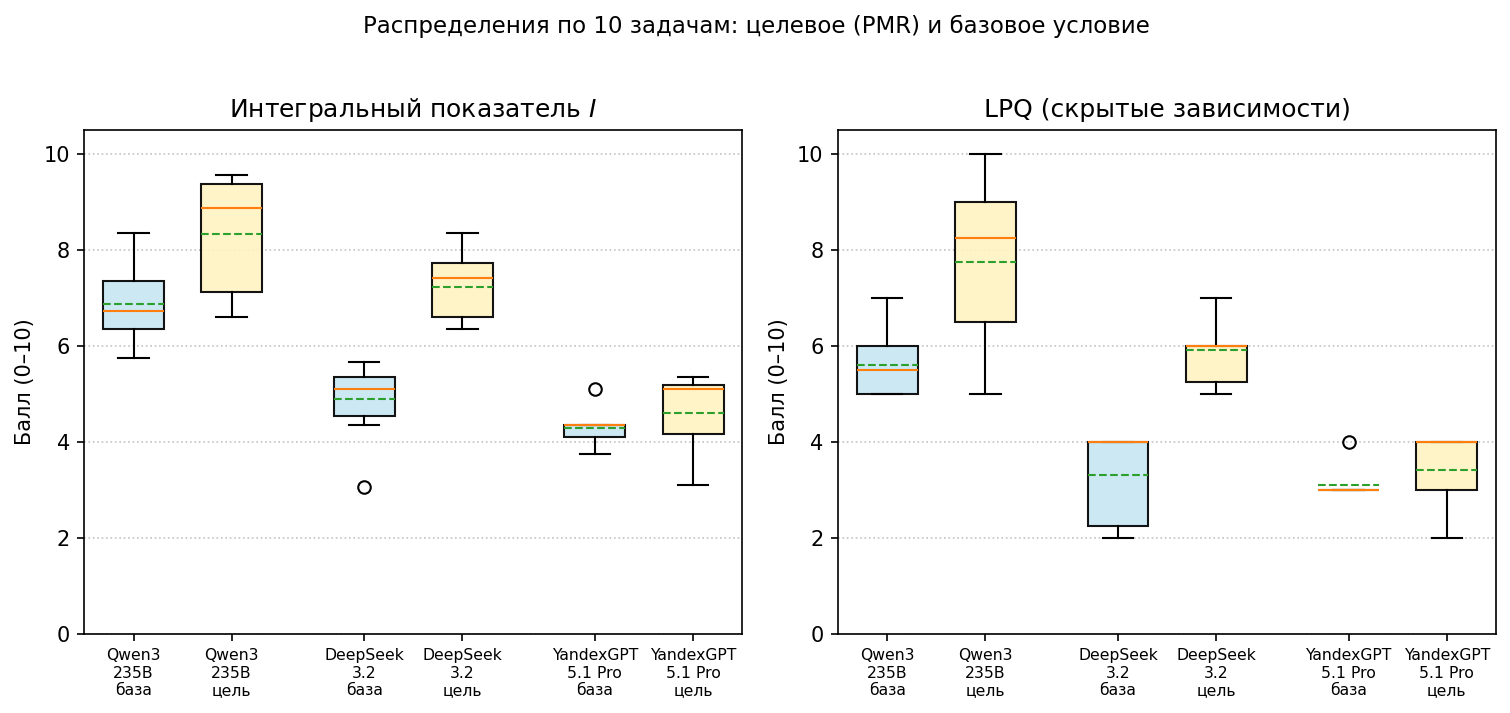
\includegraphics[width=\linewidth]{figures/pmr_I_LPQ_boxplots.png}
  \caption{Ящичковые диаграммы распределений $I$ и LPQ по десяти задачам для целевого (<<цель>>) и базового (<<база>>) условий на трёх системах. Визуально подтверждается сильнее выраженный сдвиг LPQ у Qwen3 235B и DeepSeek~3.2 и сильное перекрытие распределений $I$ у YandexGPT~5.1~Pro.}
  \label{fig:box_ilpq}
\end{figure}

Интервалы для средних по десяти задачам (табл.~\ref{tab:ci_marginal}) у Qwen3 235B и DeepSeek~3.2 не пересекаются между условиями ни по $I$, ни по LPQ, что согласуется с малыми парными $p$ в табл.~\ref{tab:paired_infer}. У YandexGPT~5.1~Pro интервалы по $I$ и LPQ существенно перекрываются, а $p_t$ и $p_W$ велики, что указывает на отсутствие устойчивого эффекта на агрегированном уровне при $n=10$.

Расщепление по уровню сложности (по пять задач в подвыборках <<промежуточный>> и <<повышенный>>) не противоречит сводной картине: для интегрального показателя у Qwen относительный прирост составляет +18\% (промежуточный) и +23\% (повышенный), для LPQ --- +33\% и +43\%; у DeepSeek для $I$ --- +42\% и +54\%, для LPQ --- +67\% и +93\%; у YandexGPT для $I$ в обеих группах +7\%, для LPQ --- +7\% и +13\%.

Наиболее выраженный относительный прирост в прогонах Qwen3 235B и DeepSeek~3.2 --- по шкале LPQ (рис.~\ref{fig:box_ilpq}). У YandexGPT~5.1~Pro эффекты малы, но сонаправлены по доменам, за исключением психотерапии, где целевой метод ниже базового на тринадцать процентов к базовому уровню (табл.~\ref{tab:aggregated}).

\subsection{Иллюстрация по задаче PMR-004}

В качестве примера качественного сопоставления условий рассмотрим задачу PMR-004 стенда PMR-Bench (домен управления): постановка требует описать процедуру приоритизации смешанного журнала требований для B2B SaaS-продукта при заданном объёме накопленных элементов и запросе руководства зафиксировать порядок работ на квартал. В прогоне Qwen3 235B автоматический судья выставил LPQ $5{,}0$ в базовом условии и $9{,}0$ в целевом; интегральный показатель --- $5{,}75$ и $9{,}4$, полнота (CMP) --- $6{,}0$ и $9{,}0$. В базовом ответе выделяется единая универсальная шкала приоритизации для всего журнала без типовой дифференциации; целевой ответ явно ветвится по четырём классам элементов (баги, функциональность, техдолг, эксперименты), для каждого класса задаются разные критерии и формулы весов, а в блоке $P$ отвергаются <<универсальные>> RICE/MoSCoW как несовместимые с разнородным бэклогом. В $E$ фиксируются точки отказа (ошибочная классификация элемента, несопоставимость шкал между классами, сдвиг стратегии 70/20/10), а в $R$ --- условия пересчёта при изменении стратегии; у базы эти развилки и критерии смены процедуры остаются имплицитными. Детальные логи и формулировка постановки доступны в открытых артефактах прогона.

\section{Обсуждение}

\subsection{Интерпретация}

Согласованный рост по шкале LPQ согласуется с тем, что явная процедурная экстернализация помогает модели формулировать неочевидные зависимости и ограничения. Больший относительный выигрыш у более мощных систем может отражать лучшее заполнение процедурного каркаса содержанием, а не только соблюдение формата.

Связь с монографией Душкина Р.~В., \textit{Метакогнитивная промпт-инженерия} [Душкин, 2025]: процедурная мета-рефлексия связывает мета-уровень (процедурная прозрачность) и уровень исполнения (артефакт); целевой промпт настоящего стенда роднится с этим требованием, а пост-ответный блок --- с линией ретроспективной фиксации контура в [Душкин, 2025]. Обобщение относительно канонической постановки \textit{Метакогнитивной промпт-инженерии} [Душкин, 2025] состоит в переносе на одноходовые не диалоговые задачи и в свёртке многоагентной декомпозиции в один промпт-контракт; сужение --- в отсутствии полного многоуровневого пайплайна из [Душкин, 2025] и в фокусе на измеримом сравнении с базовым условием на PMR-Bench.

Отрицательное относительное изменение в психотерапии у YandexGPT~5.1~Pro поддерживает рабочую гипотезу о том, что жёсткая трёхблочная структура может снижать гибкость ответа там, где ценятся нелинейность и тонкая настройка под контекст. Под гибкостью понимается операционализируемая совокупность признаков: доля содержания вне жёстких разделов и уровень практической ценности при неизменном внешнем судье. Проверка в следующем эксперименте: сравнить полную процедурную мета-рефлексию с облегчённым вариантом на поднаборе задач психотерапии при том же внешнем судье Qwen3 235B. В первичном анализе целесообразно зафиксировать относительное изменение практической ценности и интегрального показателя и при необходимости применить краткий экспертный чек-лист клинической уместности.

\subsection{Ограничения и этика}

\textbf{Внутренняя валидность.} Парный дизайн по задачам снижает дисперсию, связанную с различиями постановок, но не устраняет смещения судьи: в прогонах Qwen3 235B и DeepSeek~3.2 судья совпадал с исполнителем, что создаёт риск <<самосогласованной>> оценки формата PMR. Фиксированный порядок режимов (сначала целевой прогон всего стенда, затем базовый) не рандомизирован; возможны несезонные дрейфы API и конфигурации на стороне провайдера. Объём $n=10$ и отсутствие поправки на множественность ограничивают устойчивость $p$-значений.

\textbf{Внешняя валидность.} Три коммерческие системы не исчерпывают рынок моделей; четыре домена и десять задач не покрывают все прикладные форматы (мультиходовые диалоги, инструментальные агенты, доменно-специфичные регламенты). Перенос на другие языки постановок, другие судьи и другие веса $w_k$ требует отдельной проверки.

Этика и снижение рисков. Постановки стенда --- учебно-прикладные сценарии без идентифицируемых персональных данных; дословное цитирование ответов моделей в публичном тексте не приводится. Для возможных будущих материалов с реальными диалогами предполагаются: анонимизация и удаление идентификаторов, согласие участников при сборе данных, регламент доступа к полным логам, а для клинически чувствительных доменов --- независимая экспертная проверка уместности.

План независимой экспертизы для психотерапевтических постановок (при расширении стенда) предполагает панель из двух--трёх лицензированных клинических психологов или врачей-психиатров с опытом КПТ/ACT, слепую оценку по короткому чек-листу (клиническая уместность, безопасность, соответствие согласованному протоколу) относительно деидентифицированных текстов постановки и ответа, разрешение расхождений на консенсусной встрече и отдельное согласование с автоматическими оценками судьи. Формат --- полуструктурированная форма в веб-опроснике или таблице; сроки и размер панели уточняются при подаче гранта или партнёрства с клинической организацией.

\subsection{Направления развития}

Перспективными шагами представляются расширение набора задач, привлечение единого внешнего судьи для всех испытуемых систем, экспертная кросс-проверка автоматических оценок и сопоставление предлагаемой техники с альтернативными схемами промптинга. Отдельно целесообразна проверка гипотезы о гибкости в психотерапии по схеме, изложенной в п.~5.1.

\section{Заключение}

Вклад статьи заключается в следующем:
\begin{enumerate}
  \item Предложено операциональное описание техники процедурной мета-рефлексии (до решения, в процессе, после решения), согласованной с линией монографии Душкина [Душкин, 2025] и реализованной в одноходовой постановке открытого стенда PMR-Bench.
  \item Проведено парное сравнительное экспериментальное исследование целевого промпта и структурированного базового условия; на Qwen3 235B и DeepSeek~3.2 зафиксированы устойчивые улучшения по осям полноты (CMP), точности (ACC), глубины выявления скрытых зависимостей (LPQ) и практической ценности (PV), а также по интегральному показателю в сочетании со значимыми парными тестами при $n=10$ (табл.~\ref{tab:paired_infer}). На YandexGPT~5.1~Pro относительные приросты по агрегатам малы, парные $p$-значения велики (раздел~4).
  \item Продемонстрирована применимость метода на стенде из десяти прикладных постановок в доменах инженерии, управления, образования и психотерапии.
  \item Для воспроизводимости представлены открытый исходный код программного средства, протокол автоматического судейства и фиксация конфигураций прогонов; параметры промптинга и версии инструкций доступны в репозитории проекта (в публикацию полные тексты промптов не включались).
\end{enumerate}

Таким образом, цель и задачи, сформулированные во введении, выполнены в пилотном масштабе: операциональный контракт и схема конвейера (рис.~\ref{fig:pipeline}) изложены в разделе~3; количественное сравнение, доверительные интервалы и парные проверки для $I$ и LPQ --- в разделе~4 (табл.~\ref{tab:aggregated}--\ref{tab:ci_marginal}, табл.~\ref{tab:paired_infer}, рис.~\ref{fig:box_ilpq}). Рабочая гипотеза о приросте $I$ и LPQ подтверждается для Qwen3 235B и DeepSeek~3.2 и не подтверждается для YandexGPT~5.1~Pro на уровне агрегированных парных статистик при $n=10$; гипотеза о доминировании эффекта по LPQ согласуется с данными двух более мощных систем. Ограничения дизайна и обобщаемости сведены в разделе~5.

На стенде из десяти задач при парном дизайне показано, что целевой промпт даёт положительное относительное изменение интегрального показателя и осей качества у трёх различных испытуемых систем; наиболее выражен рост по шкале LPQ. Практическое использование --- как методический шаблон для сценариев, где важны воспроизводимость и аудит рассуждения, и как основа для расширяемого открытого стенда.

\section*{Благодарности}

Вычислительная часть работы, представленная в статье, выполнялась с использованием платформы Yandex Cloud, в частности сервисов доступа к облачным моделям генерации текста (включая API семейства YandexGPT) и сопутствующих облачных ресурсов для запуска экспериментального конвейера и обращений к внешним API моделей. Исследование проводилось при грантовой поддержке Центра Yandex Cloud по технологиям для общества. Авторы выражают благодарность команде Yandex AI Studio за инструментальную и организационную поддержку.

\section*{Список литературы}

\noindent\small При подаче в журнал, ориентирующийся на ГОСТ~Р~7.0.5 / ГОСТ~Р~7.0.100, библиографические описания ниже могут потребовать перестановки элементов, обозначения года издания электронного ресурса и замены разделителей; монография [Душкин, 2025] сохраняется в тексте и в списке в явном виде.

\begin{enumerate}
  \item Anderson J. R. The Architecture of Cognition. --- Cambridge, MA : Harvard University Press, 1983. --- 345~p.
  \item Wei J., Wang X., Schuurmans D. et al. Chain-of-Thought Prompting Elicits Reasoning in Large Language Models // NeurIPS 2022: Proceedings of the 36th International Conference on Neural Information Processing Systems. --- 2022. --- Vol.~35. --- P.~24824--24837.
  \item Yao S., Yu D., Zhao J. et al. Tree of Thoughts: Deliberate Problem Solving with Large Language Models // Advances in Neural Information Processing Systems. --- 2024. --- Vol.~36. --- P.~11809--11822.
  \item Flavell J. H. Metacognition and cognitive monitoring: a new area of cognitive-developmental inquiry // American Psychologist. --- 1979. --- Vol.~34, \textnumero~10. --- P.~906--911.
  \item Wang Y., Zhao Y. Metacognitive Prompting Improves Understanding in Large Language Models // Proceedings of the 2024 Conference of the North American Chapter of the Association for Computational Linguistics: Human Language Technologies. --- 2024. --- P.~1234--1245.
  \item Zheng L., Chiang W.-L., Ying J. et al. Judging LLM-as-a-Judge with MT-Bench and Chatbot Arena // Advances in Neural Information Processing Systems. --- 2024. --- Vol.~36. --- P.~46595--46626.
  \item Душкин Р. В. Метакогнитивная промпт-инженерия. --- Москва : ДМК Пресс, 2025. --- 238~с.
\end{enumerate}

\end{document}